\documentclass[a4paper,12pt]{article}
\usepackage{graphicx}
\usepackage{hyperref}   % use for hypertext links, including those to external documents and URLs

\begin{document}



\begin{center}
\begin{Huge}
\textbf{{\LARGE Individual Report \\ Unit Test Visualisation Project }}
\linebreak
\linebreak
\linebreak
\linebreak
\end{Huge}\end{center}




\begin{small}
\begin{flushleft}
\textbf{Author:} Keagan Phillips
\\
\textbf{Team:} Group 4
\\
\textbf{Course:} ELEN7046 - Software Technologies and Techniques
\\
\textbf{Date Submitted:} 25 June 2012
\\
\textbf{Source \& Documentation:} https://github.com/KeaganPhillips/Wit-Group-4-project
\linebreak
\linebreak
\linebreak
\linebreak
\linebreak
\end{flushleft}

\end{small}


\begin{flushleft}
\textbf{{\large Abstract}}
\end{flushleft}
This document discusses the technologies and techniques used in the development of the "Unit Test Visualisation" project. It briefly discusses the specification and proposed solution. It also highlights the individual contribution  made by the author and the group.    
\clearpage


\tableofcontents


\clearpage

\section{Introduction}
As per the ELEN 7046 course, students were required to form groups and develop a system that can be used for software visualization and/or education. Teams were given the freedom to formulate their own specification.

\subsection{Specification selection}
After much consideration the team agreed to develop a system that can visually represent unit tests to aid developers. Unit tests ensure that a system behaves in a consistent and predictable manner especially as new features are added or existing features are amended. The team however felt that the use of unit tests can be expanded to also describe software.  

\subsection{Proposed Solution}
The proposed solution was for the development of a system that can visually render class diagrams within a web browser. Upon clicking a class diagram, the developer will get the full context of each test for the selected class without having to zoom into each individual test within the code base one at a time. 


\section{Role and Responsibilities}
I assumed the lead developer role within the team. As lead developer, I had three core goals (i.e. quality, mentorship and delivery).


\subsection{Quality} 
I had to ensure that all developers conform to good coding patterns and practices by overseeing the work being done by each software engineers on the project.
\subsection{Mentorship} 
I also acted as a mentor to guide developers towards using best engineering practices while still being open to new ideas and suggestions as not to stifle creativity within the team.
\subsection{Delivery} 
Ultimately the responsibility for delivering the end product rested on my shoulders. To ensure that the system is technically sound, meet the expected requirement and that the system is delivered on time. 



\section{Individual and Group Contributions}
As developer lead I had oversight throughout the code base as a whole. I did however try not to dictate to the other developers by allowing them to be creative and to contribute meaningfully. The 'Unit Test Reflector' component was one component I worked on in isolation. The following sections briefly describe some of the core components within the system and my contribution to them.\\
\linebreak
Please refer to Figure 1 of the Group Report\cite{groupReport} for an graphical representation of the components discussed in this section.
 
\subsection{Core System Under Development}
\subsubsection{Component Overview}
This is a Microsoft Dot Net Framework 4.0\cite{dotNetFramework} console application. This application forms the core business system (i.e. The system under test). The Unit Test project is intended to target this application in order to verify it's correctness. The team did not focus to much on getting this application fully functional because it falls beyond the scope of the project. The group project focuses on the visualisation of unit tests, not the functionality of the core system under development.
\subsubsection{Test Driven Development}
This application was written in using the TDD (Test Driven Development\cite{tdd}) technique. TDD was a bit difficult to grasp for some of the team members at first, but team rapidly got used to this development technique as the project progressed.
\subsubsection{The Bank 'Demo' Application}
The group decided on a demo bank application as an illustration. Again the functionality and completeness of this project is beyond the scope of "Unit Test Visualisation". Our unit tests must have a system to test. This console bank application is therefore the test subject.
\subsubsection{Group Contribution}
All the developers on the team collectively contributed to this component. My role was to provide mentorship and to guide the other developers with respect to TDD. Because TDD was new for most developers in the group, the team decided to employ the pair programming\cite{pairprogramming} technique for the development of this project. This technique worked very well as it aided a lot in terms of rapid knowledge transfer with respect to TDD. The developers (all four) would sit together and one would write the code the TDD way. We would then rotate the developer doing the coding every few moments.

\subsection{Core System Unit Tests}
\subsubsection{Component Overview}
This compiles to a Microsoft dot Net framework 4.0\cite{dotNetFramework} .dll file. It is the test project containing automated unit tests targeting the "Core System Under Development". Test must follow the unit test coding convention\cite{codeconvention} in order for the framework to function correctly.
\subsubsection{TDD and Contributions}
TDD is a process whereby the developer first write an automated test before writing the actual application code. \\
\linebreak
All developers on the team participated in the development of this component as the team follow the TDD process. Because of the nature of TDD, the 'Core System Under Development' component and this component [Core System Unit Tests] was worked on concurrently by all developers in the team.\\
\linebreak
Again, as lead developer I played the role of mentor to guide the development team towards implementing TDD. 

\subsection{Unit Test Reflector} 
\subsubsection{Component Overview}
This component is responsible for extracting the automated unit test metadata from the "Core System Unit Tests" component. This is achieved by exploiting the "Reflection\cite{reflection}" feature of the Microsoft dot Net framework 4.0\cite{dotNetFramework}.
\subsubsection{C\# Reflection}
C\# Reflection\cite{reflection} is technique used to parse the metadata (e.g. methods, classes, types) of a compiled dll file. This is very powerful as it allows one to write code capable of reading another cosebase by inspecting the internal elements of that compiled assembly.
\subsubsection{Contribution}
The task to develop this component was assigned to me. 
\subsubsection{Test Data Structure}
As depicted in the class diagram (Figure \ref{fig1}), this component builds a C\# data structure using the metadata extracted from the unit tests. Figure \ref{fig1} shows a class diagram of the data structure it creates. This data structure consists of an array of 'ClassUnderTest' objects. Each 'ClassUnderTest' object represents a class for which we have written at least one unit test. The 'ClassUnderTest' object contains fields (i.e. public methods / public properties / class name) used to render the class diagrams on the front end canvas.\\
\linebreak
Each 'ClassUnderTest' object can have one or more 'Test' objects. And a 'Test' object can have one or more 'TestScenario' objects. Developers must write their tests using the 'Given/When/Then'\cite{gwt} technique to make tests descriptive. 
\begin{itemize}
\item \textbf{Given:} This field provides a description of the initial state of the class and it's dependencies before the test is executed.
\item \textbf{When:} This field contains a description of the event that occurs after the initial  context was created.
\item \textbf{Then:} This field provides us with the expected result(s).
\end{itemize}  

This technique allows us to extract meaningful test metadata that provide tests with more context. This data can now be sent to any output device for consumption by users. In our system we use this data structure to generate a PDF file, we bind it to an HTML 5 web front end.

\begin{center}
	\begin{figure}
		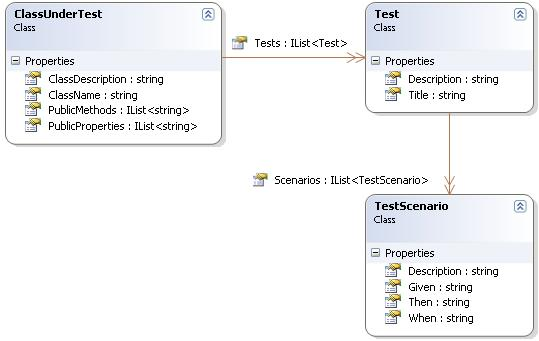
\includegraphics{classdiagram.jpg}
			\caption{}	 
			\label{fig1}    
	\end{figure}	
\end{center}



\section{Methodologies and Approach}
\subsection{Project Management}
As technical lead I have to work very closely to the project manager in the team. This is to ensure that we meet our delivery objectives on time. Please refer to Xoliswa's individual\cite{xoli} report for more project management related information. 
\subsection{Development Methodology}
The team used the Kanban methodology which falls under the 'Agile' umbrella of techniques. We used the free version of the Kanbanery\cite{kanban} tool which provides us with an online Kanban task board. Please refer to Xoliswa's individual report\cite{xoli} for more on the software development methodology.
\subsection{Source Control}
\subsubsection{Source control management system}
The team employed Git\cite{gitref} as a source control management tool. Git is a free distributed version control management system. Git was new to most members of the team at the beginning of the project, as such the team decided to use this opportunity to try out Git on this project.
\subsubsection{Source control repository}
The team chose Github\cite{github} as a central Git repository. Github\cite{github} is as service that provides developers with a centralised Git\cite{gitref} repository. Gidhub also provides developers with many useful collaboration tools and services. 
\subsubsection{Learning Git}
Learning the Git commands was a bit of a learning curve at first. The team obtained a Git 'cheatsheet' from the internet which helped the team to quickly became comfortable with the utility.\\
\linebreak
This following link is point to the teams Github repository.\\ 
\url{https://github.com/KeaganPhillips/Wit-Group-4-project}


\section{Conclusion}
The solution developed gives programmers the ability to quickly glance over a system and view all the unit test withing a project. This can be of great benefit to developers, as it gives them the full context of the internal working of a system (or a component within a system), this is especially true for new developers joining the development team as well as for junior developers allocated to the team.\\
\\
The group hence felt that the unit test visualization project fulfill both stated requirements of software visualisation and/or education.






\clearpage
\begin{thebibliography}{5}
\bibitem{dotNetFramework} .NET Framework Conceptual Overview; MSDN\\ \url{http://msdn.microsoft.com/library/zw4w595w.aspx}; Last accessed 25 June 2012

\bibitem{tdd} Introduction to Test Driven Development (TDD); Scott W. Ambler\\ \url{http://www.agiledata.org/essays/tdd.html}; Last accessed 25 June 2012

\bibitem{pairprogramming} Pair Programming; \\ \url{http://c2.com/cgi/wiki?PairProgramming}; Last accessed 25 June 2012

\bibitem{codeconvention} 'ELEN 7046 - Group Project - Unit Testing Conventions.pdf'; Keagan Phillips \\ \url{https://github.com/KeaganPhillips/Wit-Group-4-project/blob/master/Documentation/Other%20Supporting%20Documentation/ELEN%207046%20-%20Group%20Project%20-%20Unit%20Testing%20Conventions.pdf?raw=true}

\bibitem{reflection} Reflection (C\# Programming Guide); MSDN\\ \url{http://msdn.microsoft.com/en-us/library/ms173183%28v=vs.80%29.aspx}; Last accessed 25 June 2012

\bibitem{gwt} Structure your test using Given/When/Then; Dan Haywood\\ \url{http://testedobjects.sourceforge.net/m2-site/main/documentation/docbkx/html/user-guide/ch03s04.html}; Last accessed 25 June 2012

\bibitem{xoli} Xoliswa's individual report can be found at the following location\\ \url{https://github.com/KeaganPhillips/Wit-Group-4-project/tree/master/Documentation/Individual%20Reports}

\bibitem{gitref} Pro Git, by Scott Chacon, published by Apress; Publication Date: August 27, 2009; ISBN-10: 1430218339 \\ \url{http://www.amazon.com/Pro-Git-Scott-Chacon/dp/1430218339}

\bibitem{github} Gidhub source control provider\\ \url{https://github.com/}

\bibitem{groupReport} 'ELEN7046 - Group Report.pdf'\\ \url{https://github.com/KeaganPhillips/Wit-Group-4-project/blob/master/Documentation/ELEN7046%20-%20Group%20Report.pdf?raw=true}

\bibitem{kanban} Kanbanery tool used for Kanban task board\\ \url{http://kanbanery.com/}

\end{thebibliography}

 


\end{document}